\chapter{Atom} \label{ch:atom}

A la hora de decidir que editor utilizar, influye los gustos de cada uno.  Actualmente existe un catálogo enorme de editores, tanto gratuitos como de pago, los cuales ofrecen la mayoría de funcionalidades básicas que podemos esperar de en un editor.
La propia página de Ionic \footnote{\url{https://ionicframework.com/docs/v2/resources/editors_and_ides/}} nos recomiendan los siguientes basándose en el soporte que ofrecen a la hora de trabajar con este framework:
\begin{itemize}
\item Visual Studio Code
\item Atom
\item WebStorm
\item ALM
\item Angular IDE by Webclipse
\end{itemize}

\tipbox{Es importante también a la hora de elegir un editor, como se adapta este al resto de lenguajes que utilicemos, sin tener que tener abierto un editor por cada lenguaje y poder manejar con solo uno todo el proyecto.}

Para la realización de este \gls{PFC} vamos he escogido como editor Atom. Vengo usando este editor desde hace ya un tiempo no solo para programación en HTML y JS, si no también para otros lenguajes como Python o SQL y escribir textos con \LaTeX (como por ejemplo esta memoria).
Atom es un editor de código abierto para Windows, Linux y MacOS desarrollado por GitHub (el código fuente se puede descargar desde su repositorio \footnote{\url{https://github.com/atom/atom}}. Aún siendo una aplicación de escritorio, esta desarrollado utilizando tecnologías web, más concretamente Chronium y NodeJS. Esto da lugar a uno sus puntos fuertes, que es la personalización de la aplicación; como muy bien indican en su página, Atom es: \say{A hackable text editor for the 21st Century}.

\section{Instalación}

Como hemos comentado, Atom se encuentra disponible para los sistemas Windows, Linux y MacOS. Desde su propio repositorio en GitHub podemos descargarnos cualquiera de las versiones disponibles para cada uno de los sistemas antes mencionados (\url{https://github.com/atom/atom/tags}).

\section{Personalización}

Como ya se ha comentado, uno de los puntos fuertes de Atom es la personalización, permitiendo al propio usuario tener su propia configuración o utilizar recursos creados por terceros.

\subsection{Paquetes y temas}

Una característica habitual de las aplicaciones de código abierto es permitir a los usuarios crear y compartir modificaciones de la aplicación, y como no, Atom no podía ser menos. Estas modificaciones se agrupan en dos tipos:

\begin{itemize}
  \item Los \textbf{paquetes (packages)}, los cuales añaden nuevas funcionalidades al editor,
  \item y los \textbf{temas (themes)}, que cambian el aspecto visual de la aplicación.
\end{itemize}

Para ambos existe un listado donde encontrarlos en loa propia web de Atom (\url{https://atom.io/packages} y \url{https://atom.io/themes}), o más facil aún, desde la la propia configuración de la aplicación (File > Settings > Install).

\begin{figure}[H]
\centering
  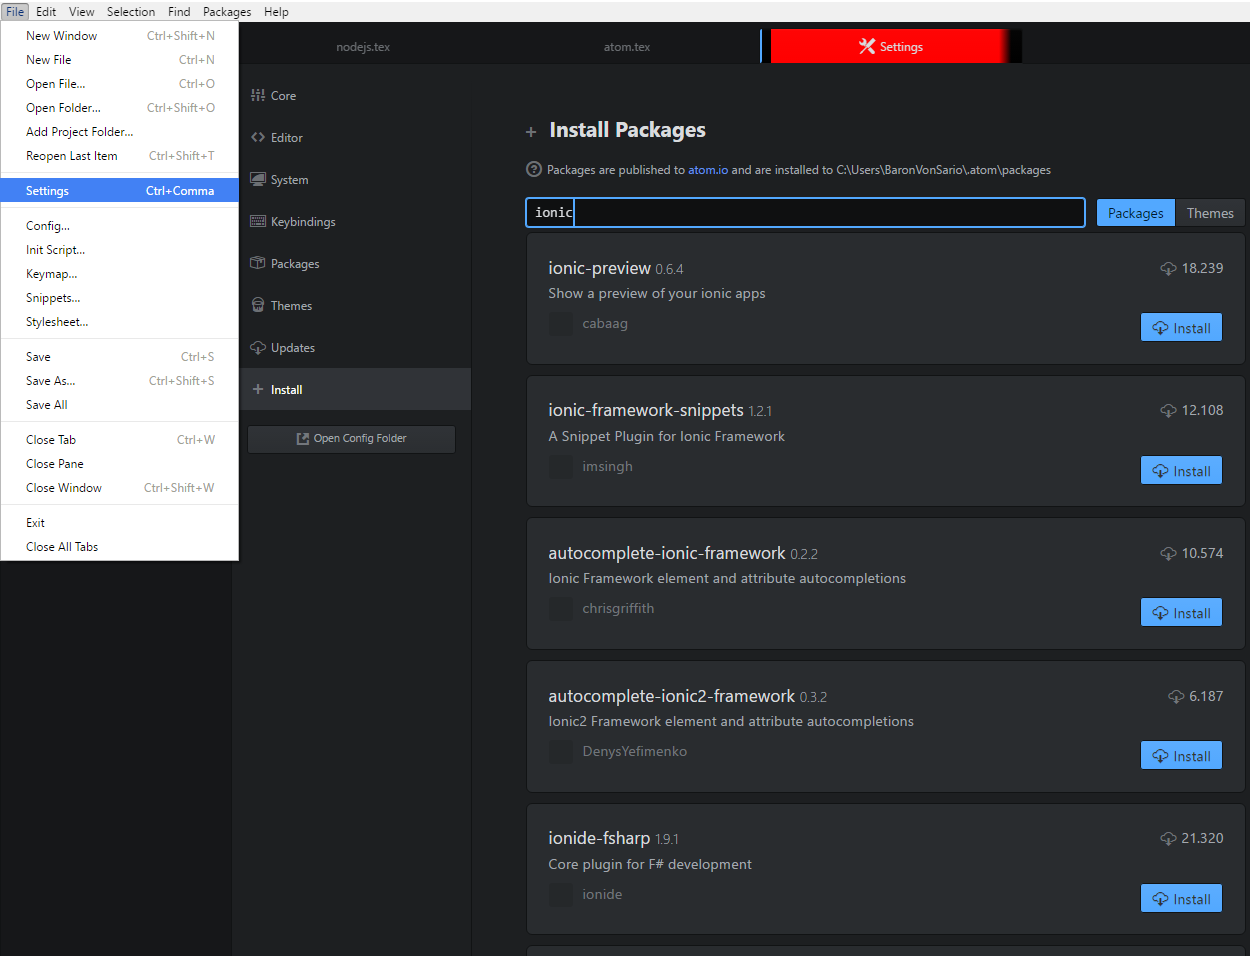
\includegraphics[width=0.8\textwidth]{Figures/anexo/anexoI/atom/install_packages_and_themes}
  \caption{Pantalla desde donde instalar paquetes y temas desde la propia aplicación de atom.}
\end{figure}
